\documentclass[pdflatex,compress,mathserif]{beamer}

%\usetheme[dark,framenumber,totalframenumber]{ElektroITK}
\usetheme[darktitle,framenumber,totalframenumber]{ElektroITK}

\usepackage[utf8]{inputenc}
\usepackage[T1]{fontenc}
\usepackage{lmodern}
\usepackage[bahasai]{babel}
\usepackage{amsmath}
\usepackage{amsfonts}
\usepackage{amssymb}
\usepackage{graphicx}
\usepackage{multicol}

\newcommand*{\Scale}[2][4]{\scalebox{#1}{$#2$}}%

\title{PEMODELAN JARINGAN KOMUNIKASI}
\subtitle{HSRP - Hot Standby Router Protocol}

\author{Tim Dosen Pengampu}

\begin{document}
	
\maketitle

\section{Network Redundancy}

\begin{frame}
	\frametitle{Network Redundancy}
	\begin{multicols}{2}
		\begin{figure}
			\centering
			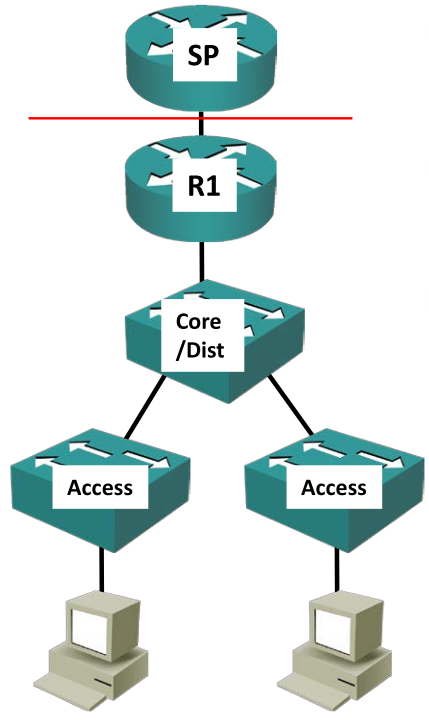
\includegraphics[height=0.8\textheight]{img/img01}
		\end{figure}
		\columnbreak
		\begin{itemize}
			\item In this example, all the network infrastructure devices
are a single point of failure
			\item If any switch or router goes down, the PCs will lose
their Internet access
			\item This is common for small branch offices where the
cost of adding redundant devices cannot be justified
		\end{itemize}
	\end{multicols}
\end{frame}

\begin{frame}{Network Redundancy}
	\begin{multicols}{2}
		\begin{figure}
			\centering
			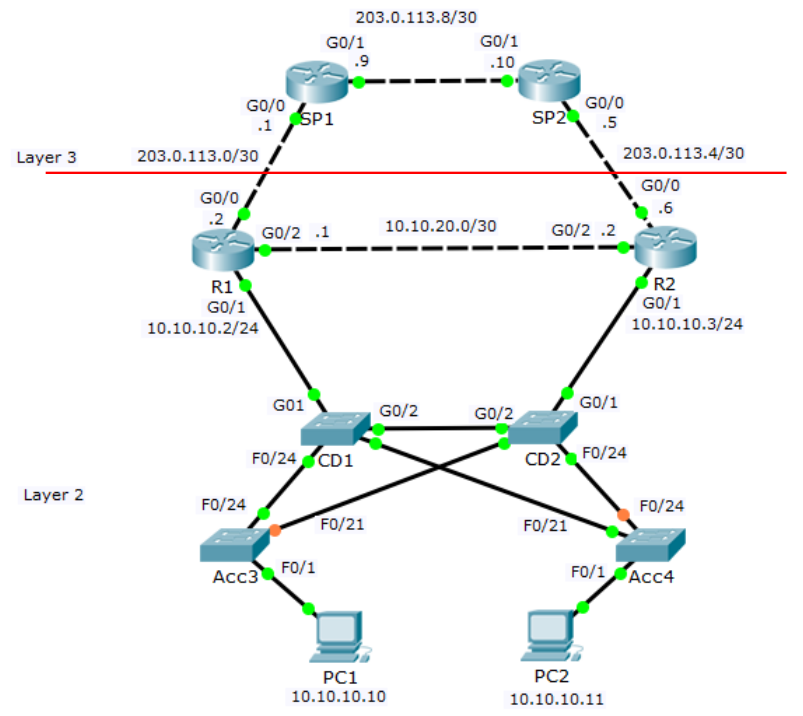
\includegraphics[width=\linewidth]{img/img02}
		\end{figure}
		\columnbreak
		\begin{itemize}
			\item The point of redundancy is to
eliminate single points of failure
			\item Now we have added redundant
switches, routers and Internet
connections
			\item We can still reach the Internet if any
core/distribution layer switch, router
or link fails
		\end{itemize}
	\end{multicols}
\end{frame}

\begin{frame}
	\frametitle{Network Redundancy – Access Layer}
	\begin{multicols}{2}
		\begin{figure}
			\centering
			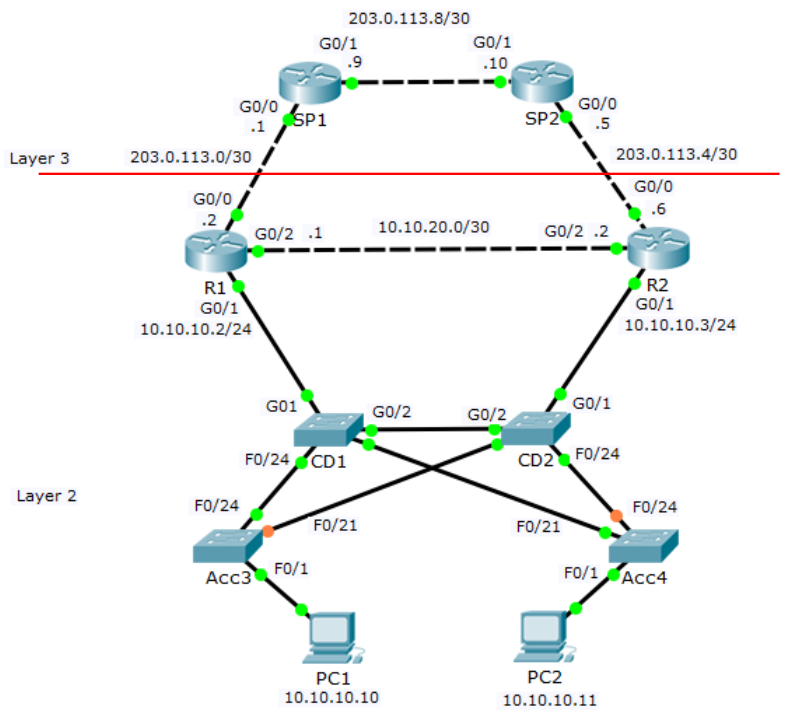
\includegraphics[width=\linewidth]{img/img03}
		\end{figure}
		\columnbreak
		\begin{itemize}
			\item We do not typically implement
redundancy at the access layer
because end hosts have only one
network card
			\item Servers with redundant NICs are an
exception
		\end{itemize}
	\end{multicols}
\end{frame}

\begin{frame}
	\frametitle{Network Redundancy}
	\begin{multicols}{2}
		\begin{figure}
			\centering
			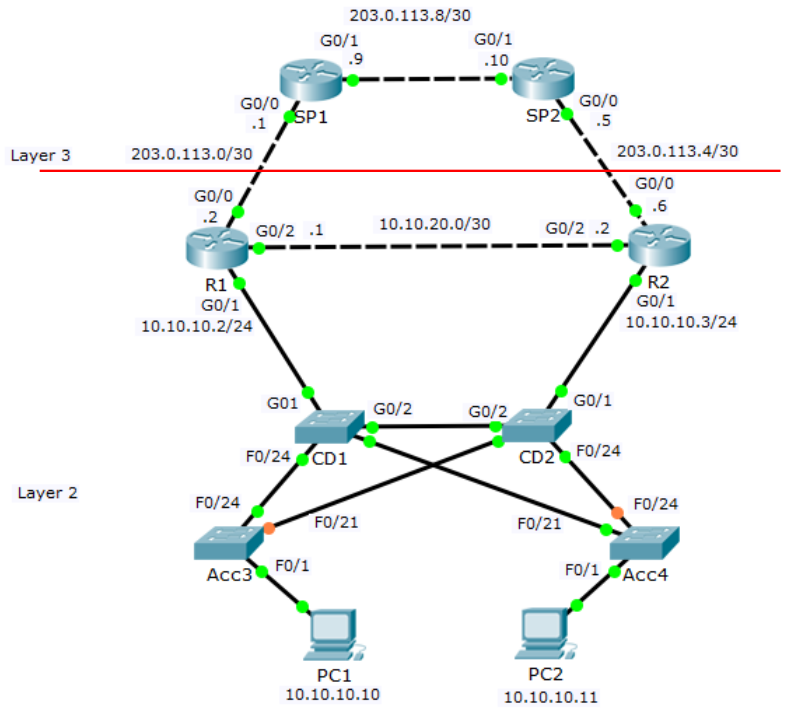
\includegraphics[width=\linewidth]{img/img04}
		\end{figure}
		\columnbreak
		\begin{itemize}
			\item In a real world network the
core/distribution layer switches
would typically be Layer 3 switches
			\item I’m using Layer 2 switches in the
example to aid learning
		\end{itemize}
	\end{multicols}
\end{frame}

\begin{frame}
	\frametitle{Network Redundancy – Layer 3 Configuration}
	\begin{multicols}{2}
		\begin{figure}
			\centering
			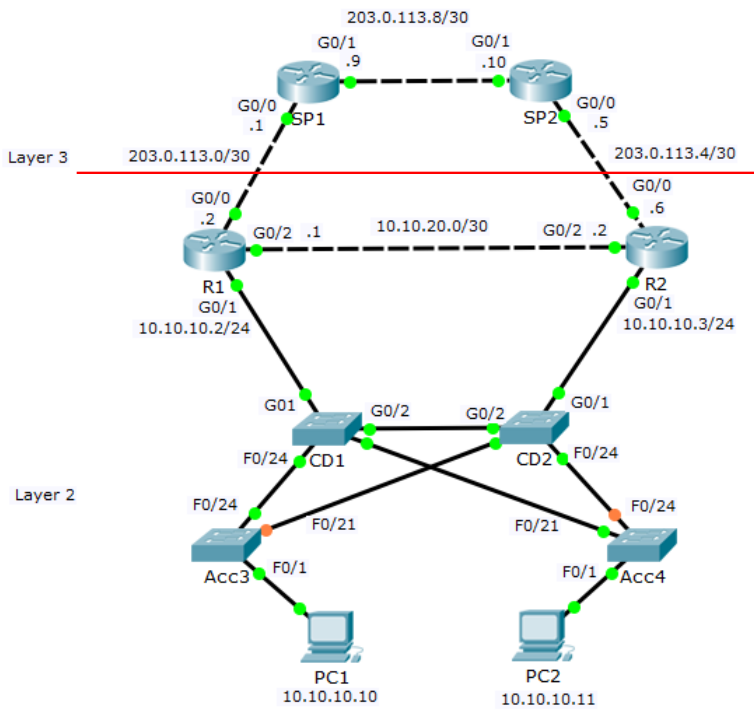
\includegraphics[width=\linewidth]{img/img05}
		\end{figure}
		\columnbreak
		\begin{itemize}
			\item Redundancy and failover are relatively
easy to implement for Layer 3 routing
			\item Routes on R1:
		\end{itemize}
		\begin{figure}
			\centering
			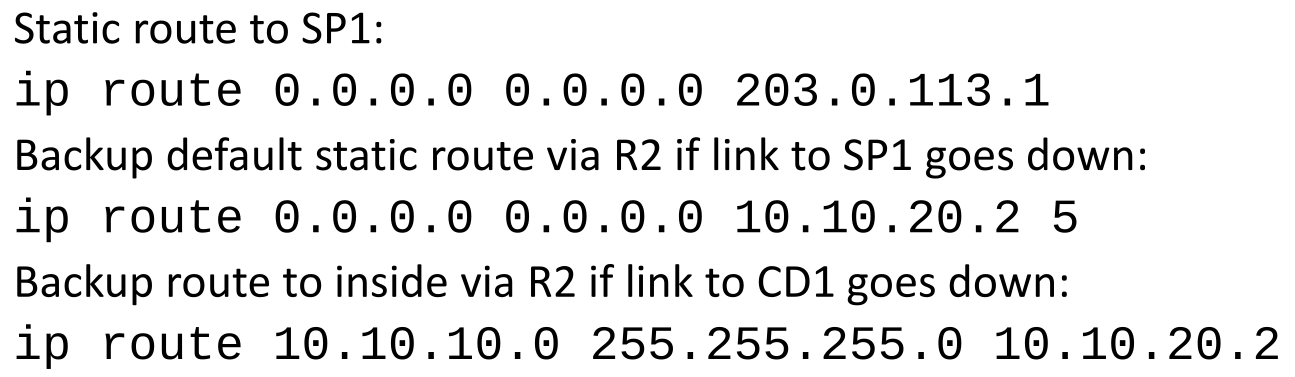
\includegraphics[height=0.3\linewidth]{img/img06}
		\end{figure}
	\end{multicols}
\end{frame}

\section{FHRP First Hop Redundancy Protocols}

\begin{frame}
	\frametitle{Network Redundancy – Layer 3 Configuration}
	\begin{multicols}{2}
		\begin{figure}
			\centering
			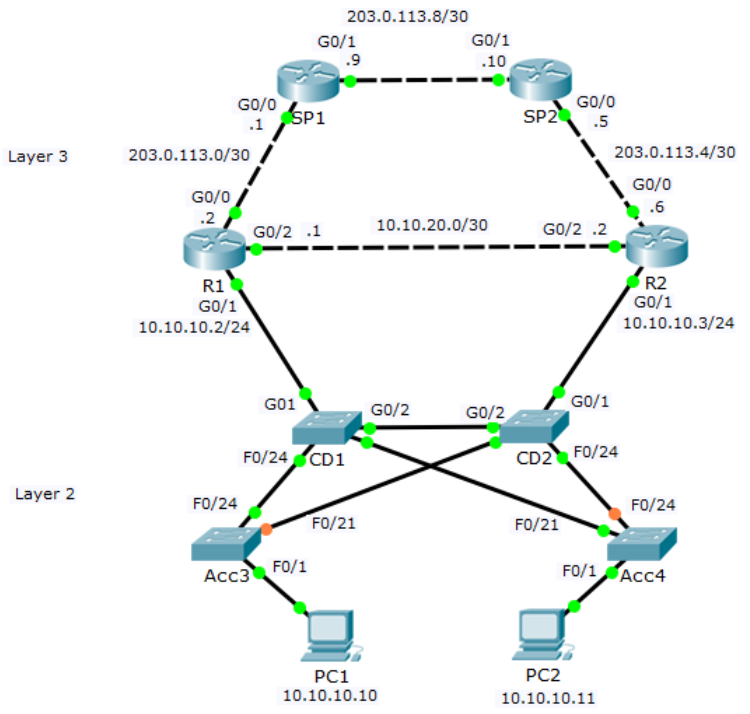
\includegraphics[width=\linewidth]{img/img07}
		\end{figure}
		\columnbreak
		\begin{itemize}
			\item Redundancy and failover are relatively
easy to implement for Layer 3 routing
			\item Routes on R1:
		\end{itemize}
		\begin{figure}
			\centering
			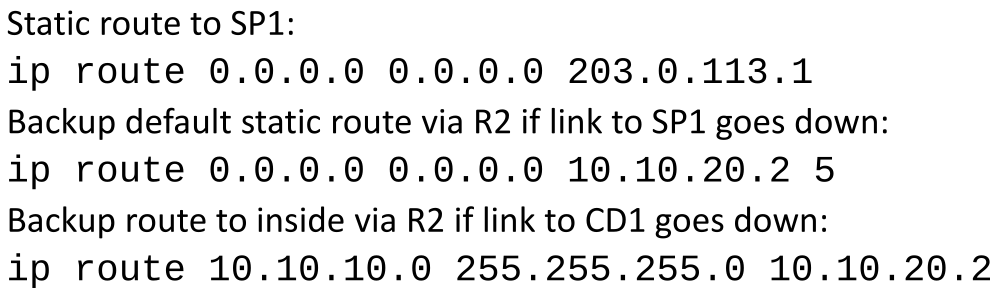
\includegraphics[height=0.3\linewidth]{img/img08}
		\end{figure}
	\end{multicols}
\end{frame}

\begin{frame}
	\frametitle{Network Redundancy}
	\begin{multicols}{2}
		\begin{figure}
			\centering
			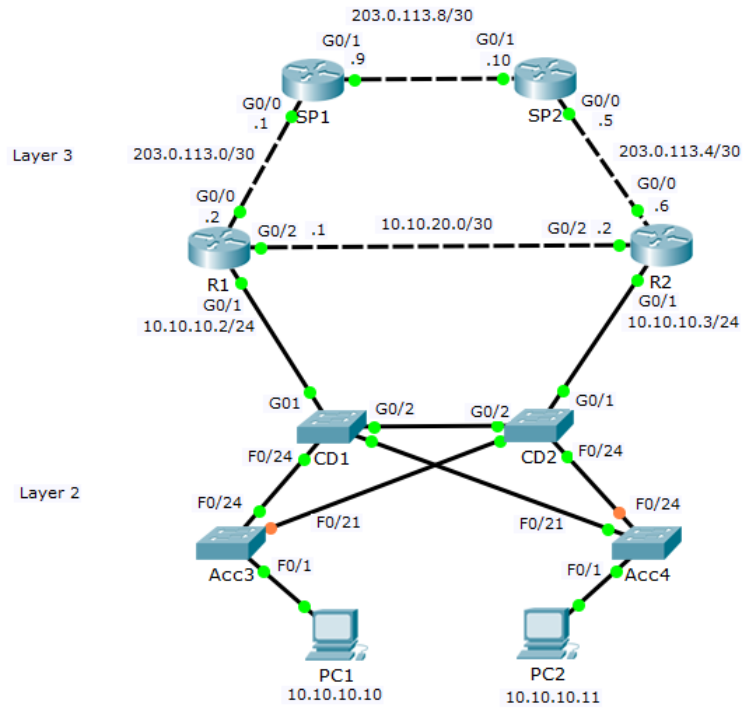
\includegraphics[width=\linewidth]{img/img09}
		\end{figure}
		\begin{itemize}
			\item We have redundant gateways for the PCs
in the 10.10.10.0/24 network:
		\end{itemize}
		\columnbreak
		\begin{itemize}
			\item R1 with IP address 10.10.10.2
			\item R2 with IP address 10.10.10.3
			\item We could configure half our PCs to use
10.10.10.2 as their default gateway, and
half to use 10.10.10.3
			\item That would be inconvenient and would
require manual reconfiguration on the
PCs to failover if one of the routers failed
		\end{itemize}
	\end{multicols}
\end{frame}

\begin{frame}
	\frametitle{First Hop Redundancy Protocols\\ (FHRP)}
	\begin{multicols}{2}
		\begin{figure}
			\centering
			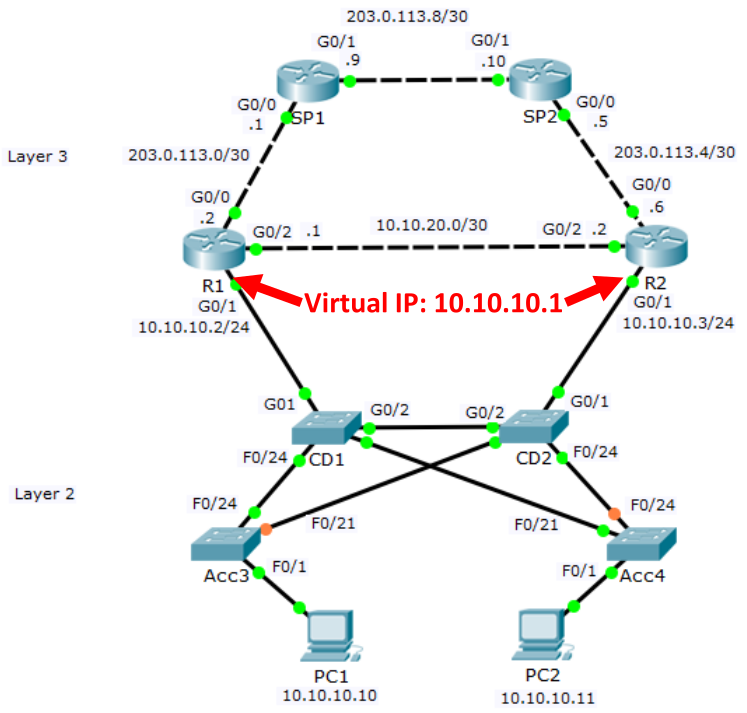
\includegraphics[width=\linewidth]{img/img10}
		\end{figure}
		\columnbreak
		\begin{itemize}
			\item First Hop Redundancy Protocols
(HSRP) use a Virtual IP (VIP) and
MAC address to allow for
automated gateway failover
			\item The hosts use the VIP as their
default gateway address
			\item If a physical gateway fails, another
gateway will take over
		\end{itemize}
	\end{multicols}
\end{frame}

\begin{frame}{First Hop Redundancy Protocols\\ (FHRP)}
	\begin{itemize}
		\item Hot Standby Router Protocol (HSRP): Cisco proprietary. Deployed in
active/standby pair.
		\item Virtual Router Redundancy Protocol (VRRP): Open standard. Deployed
in active/standby pair. Very similar to HSRP.
		\item Gateway Load Balancing Protocol (GLBP): Cisco proprietary. Supports
active/active load balancing across multiple routers.
	\end{itemize}
\end{frame}

\section{HSRP Hot Standby Router Protocol}

\begin{frame}
	\frametitle{HSRP (Hot Standby Router Protocol)}
	\begin{multicols}{2}
		\begin{figure}
			\centering
			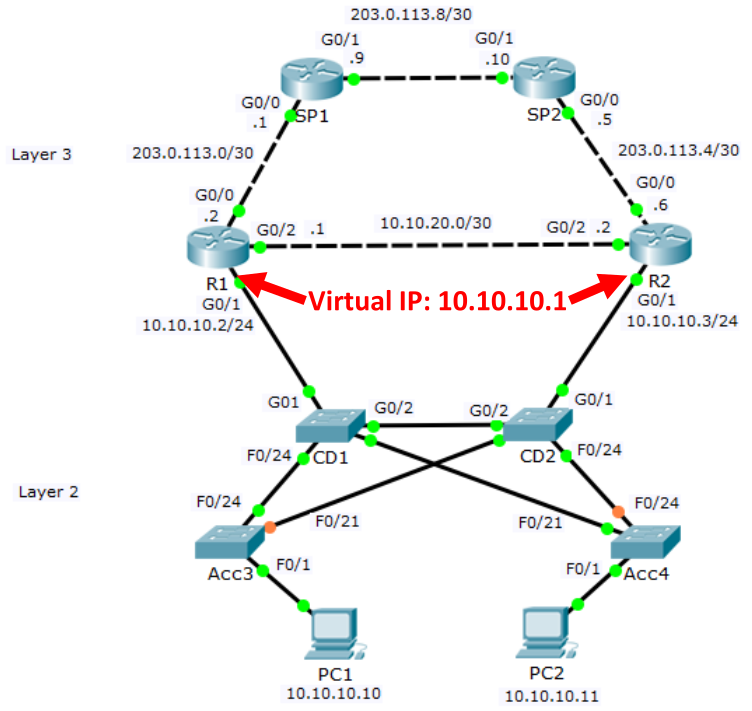
\includegraphics[width=\linewidth]{img/img11}
		\end{figure}
		\columnbreak
		\begin{itemize}
			\item HSRP uses a Virtual IP (VIP) and
MAC address to allow for
automated gateway failover
			\item The hosts use the VIP as their
default gateway address
			\item If the active gateway fails, the
standby gateway will take over
		\end{itemize}
	\end{multicols}
\end{frame}

\begin{frame}
	\frametitle{HSRP Operations}
	\begin{itemize}
		\item Both routers have a normal physical IP address and MAC address on their
HSRP interface. Unique addresses are used on both routers.
		\item They both also have the HSRP virtual IP and MAC address configured on
the interface. The same addresses are used on both routers.
		\item When they come online, one is elected the HSRP active router, the other is
the standby
		\item The active router owns the virtual IP and MAC address and responds to
ARP requests
		\item All traffic for the VIP goes through the active router
	\end{itemize}
\end{frame}

\begin{frame}{HSRP Operations}
	\begin{itemize}
		\item The routers send hello messages to each over their HSRP interface
		\item If the standby router stops receiving hellos from the active it will transition
to be the active router
		\item It will take ownership of the virtual IP and MAC address and respond to
ARP requests
	\end{itemize}
\end{frame}

\begin{frame}{HSRP Configuration}
	\begin{figure}
		\centering
		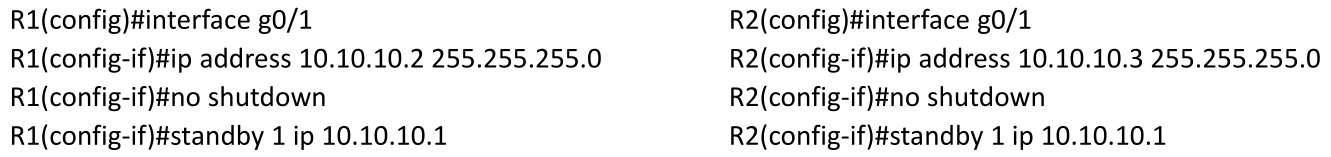
\includegraphics[width=\linewidth]{img/img12}
	\end{figure}
\end{frame}

\begin{frame}
	\frametitle{Verification – show standby}
	\begin{figure}
		\centering
		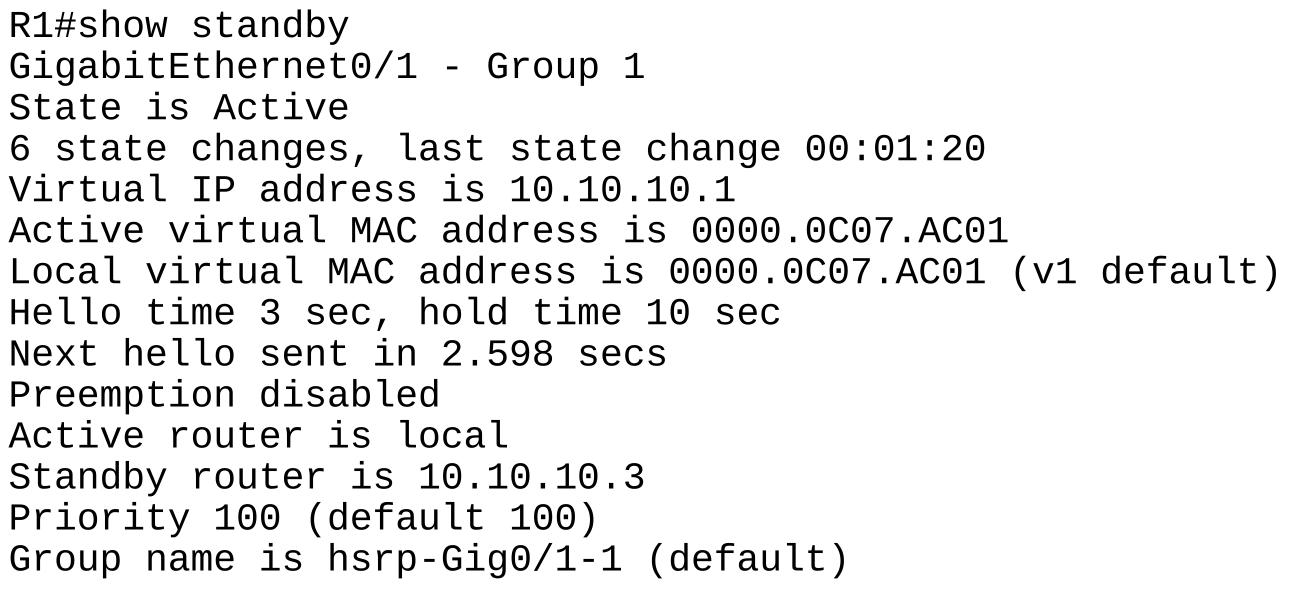
\includegraphics[width=\linewidth]{img/img13}
	\end{figure}
\end{frame}

\begin{frame}
	\frametitle{Lab}
	\begin{figure}
		\centering
		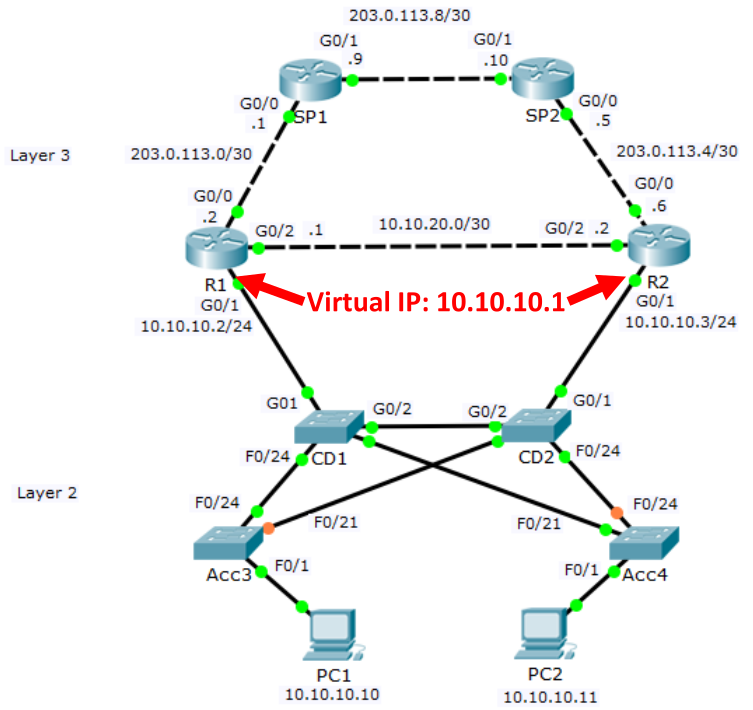
\includegraphics[height=0.8\textheight]{img/img14}
	\end{figure}
\end{frame}

\section{HSRP Advanced Topics}

\begin{frame}
	\frametitle{Priority and Pre-emption}
	\begin{itemize}
		\item You can choose which router will be the active by setting priority on the
routers
		\item The router with the higher priority will be preferred (default is 100)
		\item In the event of a tie the highest IP address wins
		\item If pre-emption is also enabled, when a higher priority router comes back
online after a failure it will transition back to active
		\item If pre-emption is not enabled (default), the lower priority router will
remain active when the failed router comes back online
		\item This can be more stable if a higher priority router is flapping
	\end{itemize}
\end{frame}

\begin{frame}
	\frametitle{HSRP Configuration - Priority and Pre-emption}
	\begin{figure}
		\centering
		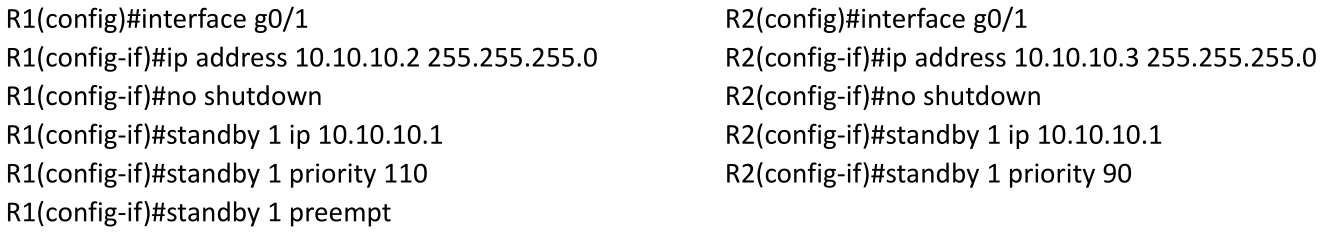
\includegraphics[width=\linewidth]{img/img15}
	\end{figure}
\end{frame}

\begin{frame}
	\frametitle{HSRP Version}
	\begin{itemize}
		\item HSRP version 2 introduced a few minor improvements
		\item The default is version 1
		\item Both routers must be running the same version
	\end{itemize}
\end{frame}

\begin{frame}
	\frametitle{HSRP Configuration - Version}
	\begin{figure}
		\centering
		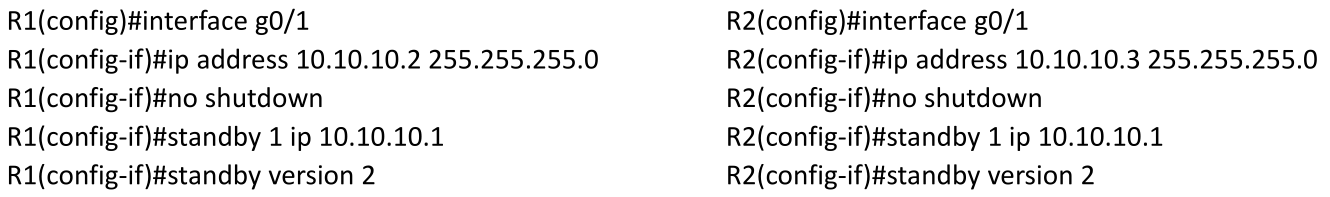
\includegraphics[width=\linewidth]{img/img16}
	\end{figure}
\end{frame}

\begin{frame}
	\frametitle{Verification – show standby}
	\begin{figure}
		\centering
		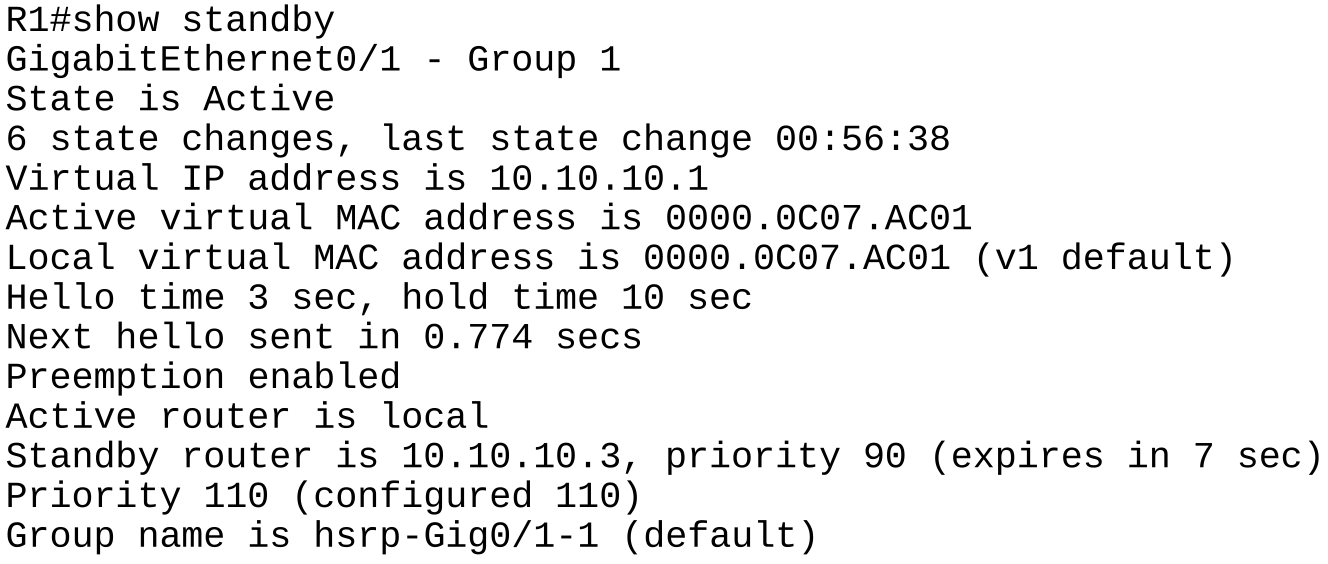
\includegraphics[width=\linewidth]{img/img17}
	\end{figure}
\end{frame}

\begin{frame}
	\frametitle{‘Active/Active’ HSRP}
	\begin{figure}
		\centering
		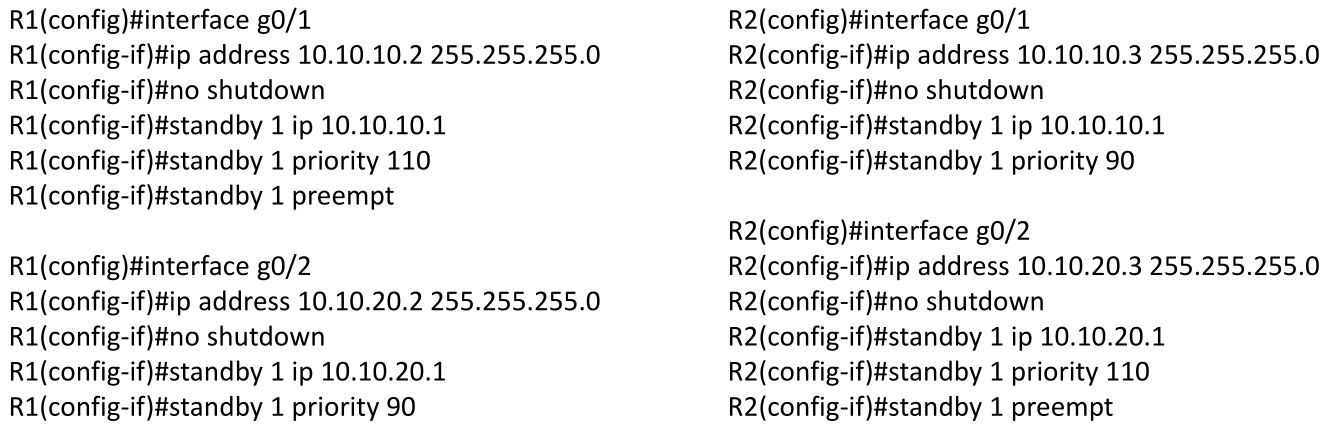
\includegraphics[width=\linewidth]{img/img18}
	\end{figure}
\end{frame}

\begin{frame}
	\frametitle{Lab}
	\begin{figure}
		\centering
		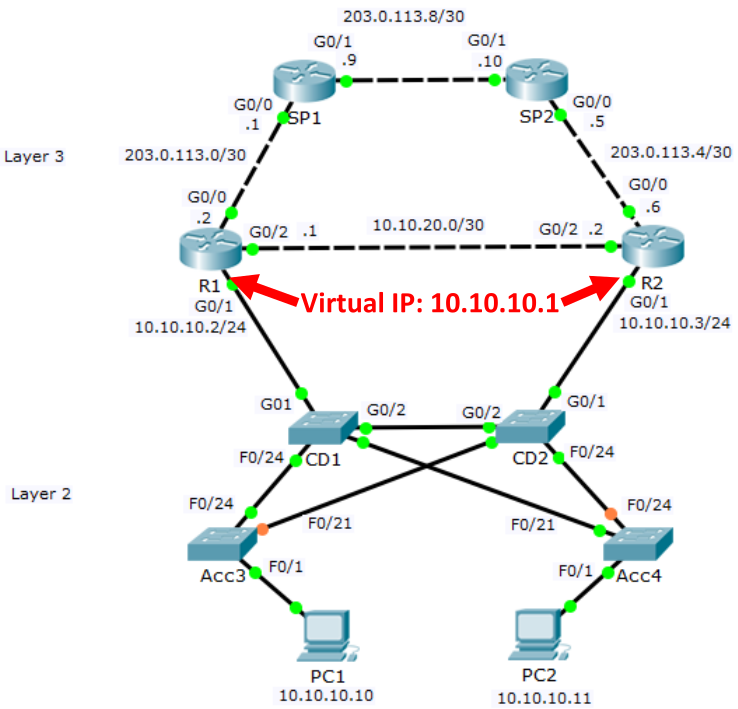
\includegraphics[width=0.6\linewidth]{img/img19}
	\end{figure}
\end{frame}

\end{document}